%-----------------------------------LICENSE------------------------------------%
%   This file is part of Mathematics-and-Physics.                              %
%                                                                              %
%   Mathematics-and-Physics is free software: you can redistribute it and/or   %
%   modify it it under the terms of the GNU General Public License as          %
%   published by the Free Software Foundation, either version 3 of the         %
%   License, or (at your option) any later version.                            %
%                                                                              %
%   Mathematics-and-Physics is distributed in the hope that it will be useful, %
%   but WITHOUT ANY WARRANTY; without even the implied warranty of             %
%   MERCHANTABILITY or FITNESS FOR A PARTICULAR PURPOSE.  See the              %
%   GNU General Public License for more details.                               %
%                                                                              %
%   You should have received a copy of the GNU General Public License along    %
%   with Mathematics-and-Physics.  If not, see <https://www.gnu.org/licenses/>.%
%------------------------------------------------------------------------------%

%   Use the standalone class for displaying the tikz image on a small PDF.
\documentclass[crop, tikz]{standalone}

%   Import the tikz package to use for the drawing.
\usepackage{tikz}

% tikz libraries used in the drawing.
\usetikzlibrary{
    angles, % Drawing angles within triangles.
    quotes  % Adding labels to angles.
}

%   Begin the document.
\begin{document}

    %   Draw the figure.
    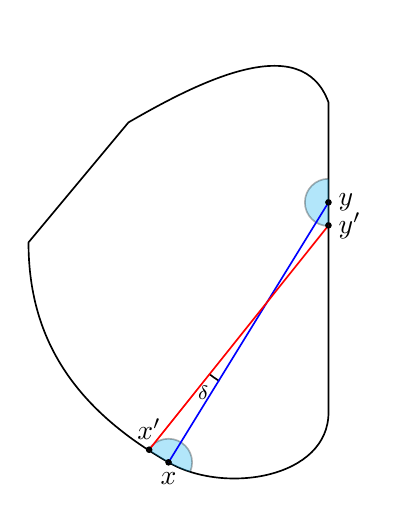
\begin{tikzpicture}[%
        line width=0.6pt,
        line cap=round
    ]
        \coordinate (x) at (-0.3in, -1.0in);
        \coordinate (y) at (0.5in, 0.3in);
        \coordinate (xp) at (-0.397in, -0.937in);
        \coordinate (yp) at (0.5in, 0.185in);
        \coordinate (O) at (0.2in, -0.19in);
        \node at (x) [below] {$x$};
        \node at (y) [right] {$y$};
        \node at (xp) [above] {$x'$};
        \node at (yp) [right] {$y'$};
        \pic[%
            draw=black,
            "\scriptsize{${\delta}$}",
            angle eccentricity=1.2,
            angle radius=1.2cm
        ]   {angle=xp--O--x};
        \draw (-1.0in, 0.1in)
            to [out=-90,in=150] (x)
            to [out=-30,in=-90] (0.5in,-0.75in)
            to [out=90,in=-90] (0.5in, 0.8in)
            to [out=110, in=30] (-0.5in, 0.7in)
            to (-1.0in, 0.1in);
        \draw[fill=black] (x) circle (0.3mm);
        \draw[fill=black] (y) circle (0.3mm);
        \draw[fill=black] (xp) circle (0.3mm);
        \draw[fill=black] (yp) circle (0.3mm);
        \clip (-1.0in, 0.1in)
            to [out=-90,in=150] (x)
            to [out=-30,in=-90] (0.5in,-0.75in)
            to [out=90,in=-90] (0.5in, 0.8in)
            to [out=110, in=30] (-0.5in, 0.7in)
            to (-1.0in, 0.1in);
        \draw[fill=cyan, opacity=0.3] (x) circle (3mm);
        \draw[fill=cyan, opacity=0.3] (y) circle (3mm);
        \draw[draw=blue] (x) to (y);
        \draw[draw=red] (xp) to (yp);
        \draw[fill=black] (x) circle (0.3mm);
        \draw[fill=black] (y) circle (0.3mm);
        \draw[fill=black] (xp) circle (0.3mm);
        \draw[fill=black] (yp) circle (0.3mm);
    \end{tikzpicture}
\end{document}
